
\chapter{Data-to-Text Generation with Custom Datasets}
\label{chap:investigating}

In this chapter, we observe and quantify behaviors of neural \acp{lm} in specific \ac{d2t} generation scenarios. To support our investigations, we venture beyond existing \ac{d2t} generation datasets.
% There are several reasons why existing datasets may not be adequate: low variability of data labels, inadequate formats, or the issues with data contamination. 
Building custom datasets helps us to overcome limitations of existing datasets and provide a more detailed picture for the task we set out to study.

In \autoref{sec:rel2text}, we examine the capabilities of \acp{plm} to describe relations between entities in knowledge graphs. As we note, existing datasets were not able to discern memorization from generalization. We thus collect a custom dataset with a large variety of relation labels, including unseen labels in the test set. Using our dataset, we investigate whether the models can correctly describe the relations they have not seen in the training data. We find out that the models can generalize unseen labels as long as the labels are human-readable and unambiguous, which is often (but not always) fulfilled in real-world data.

In \autoref{sec:quintd}, we investigate abilities of open \acp{llm} for \ac{d2t} generation. To prevent data contamination, we scrape unlabeled data from public sources across five domains. As the data is in common formats that the models have seen during pretraining, we can evaluate the ability of the models to describe the data in zero-shot settings. Using \ac{llm}-based referenceless metric and human annotators, we quantify the semantic accuracy of the generated texts with respect to the input data. We find out that although the descriptions are fluent, large majority of them contains semantic errors. We also provide practical recommendations for \ac{d2t} generation in similar scenarios.

\section{Describing Relations in Knowledge Graphs}
\label{sec:rel2text}
\begin{refbox}
    This section is based on the paper \emph{Mind the Labels: Describing Relations in Knowledge Graphs With Pretrained Models} \cite{kasnerMindLabelsDescribing2022}, joint work with Ioannis Konstas and Ondřej Dušek. The work was published in the Proceedings of the 17th Conference of the European Chapter of the Association for Computational Linguistics (EACL 2023). The project was led by the author of the thesis; Ioannis Konstas and Ondřej Dušek mentored the project.
\end{refbox}
In this section, we investigate to which extent do human-readable data labels help \acp{plm} with \ac{d2t} generation. We start by noticing that \acp{plm} can use labels such as column headings, keys, or relation names to generalize to out-of-domain examples. The question is (a) whether this ability robust enough and (b) how accurate are the outputs in cases where these labels are ambiguous or incomplete. To answer this question, we focus on the task of descibing a relation between two entities. For our experiments, we collect \textsc{Rel2Text}: a novel dataset for verbalizing a diverse set of 1,522 unique relations from three large-scale knowledge graphs (Wikidata, DBPedia, YAGO). We evaluate model outputs on unseen relations using a combination of automatic metrics and manual analysis. We find that although \acp{plm} for D2T generation expectedly fail on unclear cases, models trained with a large variety of relation labels are surprisingly robust in verbalizing novel, unseen relations. We argue that using data with a diverse set of clear and meaningful labels is key to training D2T generation systems capable of generalizing to novel domains. We release the code and data for our experiments on Github.\footnote{\url{https://github.com/kasnerz/rel2text}}


% 
% In this paper, 

\subsection{Motivation}
\ac{d2t} generation systems need to accurately capture the semantics of relations between values in the data. However, the data labels such as relation names \cite{farber2018linked,haller2022analysis}, table headings \cite{parikhToTToControlledTableToText2020}, or meaning representation keys \cite{dusekEvaluatingStateoftheartEndtoEnd2020} may provide only superficial or---if the labels are abbreviations, such as in the Rotowire dataset \cite{wiseman2017challenges}---no usable hints about the data semantics.


% \begin{figure}[t]

\begin{table}[t!] \small
    \centering
    \begin{tabular}{llp{3.7cm}l} \toprule
        \textbf{label}    & \textbf{property id}                                       & \textbf{verbalization}                                               & \textbf{note}                       \\ \midrule
        \textit{part of}  & \href{https://www.wikidata.org/wiki/Property:P361}{P361}   & \eh{} is part of \et{}.                                              & can be used verbatim                \\\cdashlinelr{1-4}
        \textit{duration} & \href{https://www.wikidata.org/wiki/Property:P2047}{P2047} & \eh{} lasted for \et{}.                                              & unambiguous verbalization           \\\cdashlinelr{1-4}
        \textit{platform} & \href{https://www.wikidata.org/wiki/Property:P400}{P400}   & \eh{} is available on \et{}.\newline\eh{} runs on \et{}.             & multiple equivalent lexical choices \\\cdashlinelr{1-4}
        \textit{occupant} & \href{https://www.wikidata.org/wiki/Property:P466}{P466}   & \et{} is occupied by \eh{}.\newline\eh{} plays at \et{}.             & semantics depends on entities       \\\cdashlinelr{1-4}
        % \textit{country}  & \href{https://www.wikidata.org/wiki/Property:P17}{P17}     & \eh{} was born in \et{}. \newline \eh{} is located in \et{}.         & semantics depends on entities       \\\cdashlinelr{1-4}
        \textit{parent}   & \href{https://www.wikidata.org/wiki/Property:P8810}{P8810} & \eh{} is the parent of \et{}. \newline \et{} is the parent of \eh{}. & ambiguous relation direction        \\\bottomrule
    \end{tabular}
    \captionof{table}{Example relation labels and the variability in their verbalizations. \eh{} and \et{} denote subject and object in the triple, respectively. The Wikidata page for each relation is available at \url{https://www.wikidata.org/wiki/Property:<property_id>}.}
    \label{tab:rel2text:example}
\end{table}

\acp{plm} such as BART \cite{lewisBARTDenoisingSequencetoSequence2019} or T5 \cite{raffelExploringLimitsTransfer2019} can quickly adapt to new domains and exhibit robustness to out-of-domain inputs. We investigate to what extent are \acp{plm} limited by the expressivity of the data labels. A suitable testing ground is the task of describing individual \acs{rdf}\glsunset{rdf} triples in a \ac{kg}, as shown in \autoref{tab:rel2text:example}. In this task, there is a wide range of lexical choices for the relation label, while the entities can be copied verbatim or with only minor morphological changes. To illustrate the problem, consider the last example in \autoref{tab:rel2text:example}: the model can use its representation of \emph{``parent''} to understand there is a \emph{``is-a-parent-of''} relation between the entities, but it has to infer (or guess) who is the parent of whom. Even in less ambiguous cases, the model still has to correctly capture the intended semantics of the relation (e.g. \emph{``occupant''} meaning \emph{``home team''}).


Current human-annotated datasets for \ac{d2t} generation are not suitable for investigating this problem, as they contain only a small number of relations and rarely contain any unseen relations in the test set \cite{mille2021automatic}. The only existing datasets covering verbalizations of a wider range of \ac{kg} relations are based on \emph{model-generated outputs} \cite{agarwalKnowledgeGraphBased2021,amaral2022wdv}.

We would also like to investigate whether incorporating long-form \emph{descriptions} of data labels helps improving model outputs. Previous works have reach contradictory conclusions: \citet{wang2021kepler} use descriptions of relations instead of their labels for relation embeddings, concluding that it results in worse performance on downstream tasks. Conversely, \citet{kale-rastogi-2020-template} and \citet{lee2021dialogue} improve the performance of their systems by including schema descriptions on the input for the dialogue state tracking and dialogue response generation systems.

Lastly, \emph{verbalizing single triples} is interesting as a stand-alone task. As we have shown previously (\Cref{sec:iterative,sec:pipeline,sec:sem-acc}), in line with other works \cite{xiangASDOTAnyShotDatatoText2022,kale-rastogi-2020-template,gupta2020infotabs,neeraja2021incorporating}, transforming triples to text helps to make the input similar to the format used during pretraining of \acp{plm}. In turn, the transformation helps with applying \acp{plm} on downstream tasks. Various methods have been tried for converting individual triples to text, ranging from simple templates and rule-based systems to prompting \acp{plm}; however, none of these works investigate how to apply these approaches to novel relations.


% 

% Using the \textsc{Rel2Text} dataset, we evalute the ability of \acp{plm} to verbalize relations which were not present in the training set. We consider both models finetuned on other relations in our dataset and models finetuned on datasets from a related domain. We also experiment with scenarios involving few-shot finetuning, training on masked labels, and extending the labels with descriptions (§\ref{sec:analysis},~\ref{sec:results}).

% We find that the \acp{plm} are quite robust in verbalizing a diverse set of relations based on their label (achieving \textasciitilde 90\% of overall entailment probability). We show that semantically unfaithful model outputs are often caused by incomplete, ambiguous, or noisy input data.



% Somewhat suprisingly, we also show that longer relation descriptions do not provide substantial improvements over using short labels.  

% However, even for data using short relation labels, the model trained on verbalizing relations can achieve results comparable to verbalizing relations using manual templates in two downstream tasks (§\ref{sec:downstream}).



\subsection{\textsc{Rel2Text} dataset}
\label{sec:rel2text:data}


For our experiments, we need data with diverse labels and their human verbalizations. We start by collecting a wide set of relations naturally occuring in three large-scale \acp{kg} (Wikidata, DBPedia, and YAGO). For each relation, we collect its label, textual description, and up to five triples in which the relation occurs in the \ac{kg}. We then use human annotatators to collect a \emph{verbalization} for each triple, i.e., a short sentence capturing the meaning of the triple. After filtering, our dataset---which we call \textsc{Rel2Text} (\underline{R}e-writing \underline{e}dge \underline{l}abels to Text),\footnote{Or simply ``Relations-to-Text''.}---contains 4,097 single triples covering 1,522 unique relations. We describe the data collection process in the following paragraphs.


\paragraph{Input Data}
An \acs{rdf} triple is a tuple $t = (s, r, o)$, where $r$ denotes the relation\footnote{In previous sections, we have also called this constituent a \emph{predicate}; these notions are equivalent.} between the subject $s$ and the object $o$.
We retrieve triples from three open large-scale \acp{kg} encoding factual knowledge:

\begin{itemize}
    \item \textbf{Wikidata} \cite{vrandevcic2014wikidata} is a large-scale Wikipedia-based \ac{kg} created using collaborative editing. With approximately 10,000 human-created relations equipped with descriptions\footnote{\url{https://www.wikidata.org/wiki/Wikidata:Database_reports/List_of_properties/all}}, it is by far the largest source of variety in relation labels.
    \item \textbf{YAGO} \cite{pellissier2020yago} is a \ac{kg} which builds upon factual knowledge from Wikidata, but uses a limited set of 116 pre-defined relations from \texttt{schema.org} \cite{guha2016schema} mapped to a subset of Wikidata relations.
    \item \textbf{DBPedia} \cite{auer2007dbpedia,lehmann2015dbpedia} is a \ac{kg} that maps Wikipedia infotables to a predefined ontology containing 1,355 relations, about 350 of which are accompanied by a description.
\end{itemize}

We query all \acp{kg} using their openly available endpoints to retrieve a list of relations in each \ac{kg}. For each relation, we retrieve up to five \textit{triples} that use this relation, and the relation \textit{description}, i.e.\ a short explanatory text.
If present, we also retrieve descriptions for the subject and the object.

We apply a set of filtering heuristics, leaving out e.g.\ relations describing \ac{kg} metadata or identification numbers.\footnote{Relations describing various IDs make up a large portion of relations in Wikidata. Since we focus on diversity instead of coverage, we decided not to include these relations in our dataset.} In this way, we collect 7,334 triples with 1,716 relations in total.

\paragraph{Annotation Process}
We collect human-written verbalizations for all input triples using Prolific.\footnote{\url{https://www.prolific.co/}} We built a web interface in which the human annotators are shown a single triple $t$ and asked to describe it in a single sentence. The annotators are encouraged to re-use the entities in their original form, but they are able to change the form if necessary. The annotators can also report noisy inputs. We employed 420 annotators in total, each of which annotated 20 examples. We set the average reward per hour according to the platform recommendations to  \textsterling{}7.29 per hour and we accepted all the inputs which passed our built-in checks.

\paragraph{Postprocessing the Data}
A considerable portion of the collected verbalizations contain typos and grammatical errors, misunderstood meaning of the relation, or extra information in the input. To ensure high quality of our data, we manually examined all crowdsourced examples and annotated them as \textit{OK}, \textit{noisy}, \textit{corrupted} or \textit{containing extra information}. For our experiments, we only use the subset of our dataset with \textit{OK} annotations, one per input triple (4,097 examples, 1,522 distinct relations).


\section{Analysis and Evaluation}
In our analysis, we are interested in the following research questions:
\begin{itemize}
    \item \textbf{RQ1:} Are the PLMs finetuned for D2T generation able to describe relations \textit{not present in the finetuning corpus}?
    \item \textbf{RQ2:} How many \textit{training examples} do the PLMs need to generate satisfactory outputs?
    \item \textbf{RQ3:} How do the PLMs behave when provided \textit{limited lexical cues} about the relation?
    \item \textbf{RQ4:} Can relation \textit{descriptions} help to clarify ambiguous cases and improve semantic accuracy of the outputs?
\end{itemize}

To answer these questions, we divide our \textsc{Rel2text} dataset into a training and test splits (see §\ref{sec:setup} for details). We then use the \textbf{\textsc{Rel2Text} test set} to evaluate a finetuned BART model \cite{lewis2020bart}, a pretrained encoder-decoder transformer, which is used as a backbone of many recent data-to-text models (\citealp{ke2021jointgt,xing2021structure,ribeiro2020investigating,liu2021kg}).\footnote{We believe that our findings also apply to similar models such as T5 \cite{raffel2020exploring}, which have shown comparable performance on related tasks.}

To answer \textit{RQ1}, we compare the performance of BART finetuned on the \textsc{Rel2Text} training set with BART finetuned on two qualitatively different D2T datasets -- \textsc{WebNLG} and \textsc{KeLM}. Using \textsc{Rel2text} only, we then prepare various setups for answering \textit{RQ2}, \textit{RQ3}, and \textit{RQ4} (details in §\ref{sec:experiments}). We analyze the outputs of the models  both automatically (§\ref{sec:auto}) and manually (§\ref{sec:manual}).



\subsection{Experimental Setup}
\label{sec:setup}

\paragraph*{Datasets}  We experiment with the following datasets, all of which focus on verbalizing factual information from KGs and use the same triple-based input data format:
\begin{itemize}
    \item \textsc{Rel2Text}. Our dataset (cf.\ §\ref{sec:rel2text}) with single triples from three KGs with 4,097 examples, 1,522 relations and \textit{human-annotated} outputs.
    \item \textsc{WebNLG} \cite{ferreira20202020,gardent2017webnlg}. A DBPedia-based triple-to-text dataset with 38k examples, 411 relations, up to 7 triples per example, and \textit{human-annotated} outputs. We use the English part of version 3.0 from HuggingFace.\footnote{\url{https://huggingface.co/datasets/web_nlg}}
    \item \textsc{KeLM} \cite{agarwal2021knowledge}. A Wikidata-based dataset with 11M examples, 1,519 relations, up to 13 triples per example, and \textit{model-generated} outputs. We use the dataset released by the authors, splitting it in a 1:100 ratio into validation and training data.
\end{itemize}

\paragraph{Rel2Text Data Split} We use approximately 15\% of the \textsc{Rel2Text} examples for the \textbf{test set}. To ensure maximum fairness and focus on model generalization to unseen relations, we do not include in the \textsc{Rel2Text} test set any relations which have an exact string match with a relation in \textsc{KeLM}, \textsc{WebNLG}, or the \textsc{Rel2Text} training set. We also exclude any relations for which the maximum semantic similarity\footnote{Computed as cosine similarity between embeddings of the labels, which are encoded using \texttt{all-distilroberta-v1} from SBERT \cite{reimers-2019-sentence-bert}.} to any \textsc{KeLM}/\textsc{WebNLG}/\textsc{Rel2Text} training relation exceeds a threshold of $0.9$. We set this threshold empirically in order to exclude relations which are almost synonymous, but slightly lexically different.
We use 90\% of the remaining examples for the training set and 10\% for the validation set.

\paragraph{Data Preprocessing} We split the camel case in the relation labels. For finetuning the models, we linearize the input triples by marking the triple constituents with special tokens \textit{<head>}, \textit{<rel>} and \textit{<tail>}, which we add to the model vocabulary.

\paragraph{Training and Decoding Setup} In a default scenario, we finetune BART\textsc{-base} for 10 epochs and select the best checkpoint using validation BLEU score, then use greedy decoding to produce outputs. We repeat each experiment with five random seeds, averaging the results. See Appendix~\ref{app:hyperparams} for details.


\subsection{Compared Systems}
\label{sec:experiments}
\paragraph{Copy Baseline} We introduce a simple baseline by outputting the triple constituents separated by space: ``$e_h\text{ }r\text{ }e_t$''.



\paragraph{Full Training Data} We use the default setup (§\ref{sec:setup}) on full \textsc{Rel2Text} and \textsc{WebNLG} training sets. For \textsc{KeLM} (which is about 300$\times$ larger than WebNLG), we finetune the model for 1 epoch only. We denote the trained models \BARTr{}, \BARTw{}, and \BARTk{}, respectively.

\paragraph{Limited Training Data} For the limited training data setup, we prepare few-shot splits from \textsc{Rel2Text} as subsets containing $N=$ \{25, 50, 100, 200\} relations with a single example per relation. We select examples at random, ensuring that each few-shot split is a subset of the larger splits. We finetune the \textit{fewshot-N} models for 10 epochs without validation, using the last checkpoint.

\paragraph{Limited Lexical Cues} In D2T datasets (with certain exceptions, cf.\ \citet{gardent2017creating}), unclear labels are kept in original form, implicitly assuming that the models will learn the verbalizations from the training data. We investigate how the models behave if we take this issue to the extreme, i.e. if the relation labels are not available at all. We consider three scenarios:
\begin{itemize}
    \item \textit{mask-test} -- We train the model on \textsc{Rel2Text} in the standard training setup. For testing, we replace the relation labels in  \textsc{Rel2Text} with the \textit{<mask>} token.
    \item \textit{mask-train} -- For training, we replace the relation labels in  \textsc{Rel2Text} with the \textit{<mask>} token. We test the model on \textsc{Rel2Text} in the standard evaluation setup.
    \item \textit{mask-all} -- We replace the relation labels in  \textsc{Rel2Text} with the \textit{<mask>} token for both training and testing.
\end{itemize}


\paragraph{Incorporating Descriptions} Our dataset contains short textual descriptions of the relations, which may be useful to disambiguate its meaning and provide additional cues to the model. We consider two scenarios:
\begin{itemize}
    \item \textit{desc-repl} -- We replace the relation label with its description.
    \item \textit{desc-cat} -- We concatenate the relation description with the input, separated using the special token \textit{<rel\_desc>}.
\end{itemize}



\begin{table*}[!htp]\centering
    \footnotesize
    \setlength{\tabcolsep}{5pt}
    \begin{tabular}{@{}lc>{\hspace{-2mm}}c>{\hspace{-2mm}}c>{\hspace{-2mm}}cc>{\hspace{-2mm}}c>{\hspace{-2mm}}c>{\hspace{-2mm}}c>{\hspace{-2mm}}cc>{\hspace{-2mm}}c>{\hspace{-2mm}}c>{\hspace{-2mm}}c>{\hspace{-2mm}}c@{}}\toprule
        \multirow{2}{*}{} & \multicolumn{3}{c}{\textbf{Lexical}} & \multicolumn{5}{c}{\textbf{Semantics}} & \multicolumn{5}{c}{\textbf{Referenceless}}                                                                                              \\\cmidrule(r){2-4}\cmidrule(r){5-9}\cmidrule{10-14}
                          & \bf BLEU                             & \bf MET                                & \bf BLR                                    & \bf SS & \bf C & \bf N & \bf E & \bf NB & \bf U-1 & \bf CE-2 & \bf TTR & \bf PPL & \bf len \\\midrule
        \it human         & -                                    & -                                      & -                                          & -      & -     & -     & -     & -      & 1785    & 2.13     & 0.62    & 5.88    & 9.55    \\
        \it copy          & 29.04                                & 37.52                                  & 0.09                                       & 4.79   & 1.22  & 7.57  & 91.21 & 0.74   & 1606    & 1.17     & 0.7     & 7.55    & 6.72    \\\hdashline[0.5pt/2pt]
        \it \BARTr{}      & 52.54                                & 44.86                                  & 0.54                                       & 4.72   & 3.50  & 4.65  & 91.85 & 0.88   & 1661    & 1.96     & 0.58    & 5.89    & 9.16    \\
        \it \BARTw{}      & 41.99                                & 41.59                                  & 0.41                                       & 4.65   & 3.68  & 6.93  & 89.39 & 0.86   & 1651    & 2.54     & 0.56    & 5.65    & 10.29   \\
        \it \BARTk{}      & 46.74                                & 42.94                                  & 0.46                                       & 4.70   & 3.95  & 5.29  & 90.77 & 0.86   & 1652    & 2.32     & 0.56    & 5.83    & 9.71    \\\hdashline[0.5pt/2pt]
        \it fewshot-25    & 31.13                                & 35.52                                  & -0.02                                      & 3.94   & 8.35  & 27.26 & 64.39 & 0.65   & 1445    & 2.93     & 0.52    & 5.34    & 10.67   \\
        \it fewshot-50    & 40.60                                & 40.05                                  & 0.25                                       & 4.44   & 8.04  & 13.12 & 78.84 & 0.76   & 1536    & 2.31     & 0.55    & 5.79    & 9.90    \\
        \it fewshot-100   & 45.88                                & 42.38                                  & 0.38                                       & 4.53   & 6.34  & 10.60 & 83.06 & 0.81   & 1600    & 2.13     & 0.57    & 5.85    & 9.57    \\
        \it fewshot-200   & 48.67                                & 43.34                                  & 0.44                                       & 4.58   & 5.40  & 9.03  & 85.57 & 0.83   & 1626    & 2.04     & 0.58    & 5.89    & 9.36    \\\hdashline[0.5pt/2pt]
        \it mask-test     & 42.45                                & 38.52                                  & 0.25                                       & 3.99   & 14.91 & 18.47 & 66.62 & 0.65   & 1669    & 1.96     & 0.61    & 5.69    & 8.96    \\
        \it mask-train    & 46.90                                & 43.15                                  & 0.43                                       & 4.55   & 5.85  & 11.55 & 82.61 & 0.81   & 1646    & 2.00     & 0.57    & 5.91    & 9.74    \\
        \it mask-all      & 42.53                                & 38.49                                  & 0.24                                       & 3.85   & 17.58 & 25.15 & 57.26 & 0.61   & 1677    & 1.96     & 0.61    & 5.66    & 9.16    \\\hdashline[0.5pt/2pt]
        \it desc-repl     & 49.35                                & 42.85                                  & 0.47                                       & 4.57   & 5.78  & 8.80  & 85.42 & 0.82   & 1693    & 1.94     & 0.59    & 5.86    & 9.18    \\
        \it desc-cat      & 53.07                                & 45.04                                  & 0.55                                       & 4.72   & 3.46  & 4.66  & 91.88 & 0.87   & 1668    & 1.91     & 0.59    & 5.92    & 9.11    \\
        \bottomrule
    \end{tabular}
    \caption{The summary of evaluation using automatic metrics on \textsc{Rel2text} test set. \textbf{MET} = METEOR, \textbf{BLR} = BLEURT, \textbf{TTR} = MSTTR. See §\ref{sec:setup} for the descriptions of the models, §\ref{sec:auto} for the descriptions of the metrics, and Table \ref{tab:autostdev} for standard deviations.}
    \label{tab:auto}
\end{table*}


\subsection{Automatic Evaluation}
\label{sec:auto}
To get a high-level overview of model behavior, we evaluate generated outputs using the GEM-metrics\footnote{\url{https://github.com/GEM-benchmark/GEM-metrics}} package \cite{gehrmann2021gem}, which provides an extensive set of automatic metrics for text generation.

\paragraph{Lexical Similarity} We first measure lexical similarity between the model outputs and human references using \textbf{BLEU} \cite{papineni2002bleu}, \mbox{\textbf{METEOR}} \cite{banerjee-lavie-2005-meteor}, and \textbf{BLEURT} \cite{sellam2020bleurt}. The first two metrics focus on n-gram overlap; the latter is a trained metric that also captures semantic similarity between the output and the reference. Although these metrics should not be used in isolation \cite{gehrmann2022repairing}, they give us a better overview of the output quality in combination with other metrics.

\paragraph{Semantic Similarity and Legibility} Lexical similarity metrics focus on the surface form, which may not be telling the whole story. For example, if the relation \mbox{\textit{parent}} denotes that $e_t$ \textit{is the parent of} $e_h$, but the entities are swapped in the generated text, the output will be incorrect, although lexical similarity metrics will be high. To get deeper insights into semantic and lexical properties of the outputs, we use NUBIA \cite{kane2020nubia}, which is a trained metric combining several features to measure ``interchangeability'' (equivalence) of two texts. The metric outputs a single score (\textbf{NB}) with a value between 0 and 1. We also report its individual underlying features:
the semantic similarity score (\textbf{SS}) on a 0-5 scale, predicted by RoBERTa \cite{liu2019roberta} finetuned on the STS-B benchmark \cite{cer-etal-2017-semeval}; the contradiction (\textbf{C}), neutral (\textbf{N}), and entailment (\textbf{E}) probabilities from RoBERTa finetuned on the MNLI challenge from the GLUE benchmark \cite{wang2018glue}; and the perplexity score (\textbf{PPL}) from vanilla GPT-2 \cite{radford2019language}, computed as a geometric mean of probabilities of the tokens in each step (this score is referenceless).


\paragraph{Lexical Diversity} To assess lexical diversity of the generated texts, we use several metrics used in previous work \cite{duvsek2020evaluating_challenge,van2018measuring}. We measure the number of unique n-grams (\textbf{U-1}), conditional entropy of bi-grams (\textbf{CE-2}), and the mean segmental type-token ratio over segment lengths of 100 (\textbf{MSTTR}; \citealp{johnson1944studies}). We also measure the average output length in tokens (\textbf{len}).

\begin{table*}[ht]
    \centering\footnotesize
    % \setlength{\tabcolsep}{4pt}
    % \renewcommand{\arraystretch}{1.25}
    \begin{tabular}{@{}p{0.5cm}p{0.8cm}p{12cm}@{}} \toprule

         & \textbf{Lbl} & \textbf{Example inputs and outputs (\red{\xmark} incorrect, \green{\cmark} correct)}                                                                                                                                                                                    \\ \midrule
        %
        \multirow{12}{*}{\rotatebox[origin=c]{90}{\textit{model}}}
        % 
         & \textsc{Sem} & \emph{(Yousra Matine, sport country, Morocco)} \newline \red{\xmark} Yousra Matine was born in Morocco. [\emph{mask-mask}] \newline  \green{\cmark} Yousra Matine plays for Morocco. [\BARTr]                                                                           \\[2mm]
         & \textsc{Dir} & \emph{(Kentucky Channel, former broadcast network, KET ED)} \newline \red{\xmark} KET ED was broadcast on Kentucky Channel ED. [\emph{fewshot-100}] \newline  \green{\cmark} The Kentucky Channel was broadcast on KET ED. [\BARTr]                                     \\[2mm]
         & \textsc{Lit} & \emph{(Vietnam Television, first air date, 1970-09-07)} \newline \red{\xmark} The first air date of Vietnam Television was 1970-09-07. [\BARTk] \newline  \green{\cmark} Vietnam Television first aired on 1970-09-07. [\BARTr]                                         \\[2mm]
         & \textsc{Lex} & \emph{(RPG-43, used in war , The Troubles)} \newline \red{\xmark} RPG-43 was used in the The Troubles. [\BARTr] \newline  \green{\cmark} The RPG-43 was used in the Troubles. [\BARTk]                                                                                  \\[1mm]\hdashline[0.5pt/2pt]\\[-3mm]
        %
        \multirow{6}{*}{\rotatebox[origin=c]{90}{\textit{data}}}
        %
         & \textsc{Ent} & \emph{(The Age of Entitlement, by artist, The Basics)} \newline \red{\xmark} The Age of Entitlement was written by The Basics. [\BARTk] \newline  \green{\cmark} The Age of Entitlement was recorded by The Basics.  [\BARTr]                                           \\[2mm]
         & \textsc{Lbl} & \emph{(General Motors Epsilon platform, vehicle, Cadillac XTS)} \newline \red{\xmark} General Motors Epsilon is a vehicle similar to the Cadillac XTS. [\BARTw] \newline  \green{\cmark} General Motors Epsilon platform is used in the Cadillac XTS. [\emph{desc-cat}] \\
        \bottomrule
    \end{tabular}
    \caption{Error categories used in manual analysis, with examples of errors found and corresponding correct verbalizations.
        Model error types (top):
        \textsc{Sem} -- The output is semantically incorrect,
        \textsc{Dir} -- The direction of the relation is swapped,
        \textsc{Lit} -- The verbalization is too literal,
        \textsc{Lex} -- There is a lexical error in the output.
        %
        Input data error types (bottom):
        \textsc{Ent} -- The verbalization may depend on the entities,
        \textsc{Lbl} -- The relation label is not clear.
    }
    \label{tab:rel2text:cat}
\end{table*}


\subsection{Manual Error Analysis}
\label{sec:manual}
To examine the sources of errors, we perform an in-house annotation of the model outputs.
We identify four model error types based on preliminary observations:
semantic errors (\textsc{Sem}), with a swap of the relation direction
(\textsc{Dir}) as a special case, too literal (\textsc{Lit}), i.e.\ containing awkward or misleading phrasing, and grammar/lexical errors (\textsc{Lex}). We further annotate two types of input data errors: ambiguous relations (\textsc{Ent}) and relations with unclear labels (\textsc{Lbl}).
Examples are shown in Table~\ref{tab:cat}.
%
We select 100 random examples together with their corresponding outputs from the \textit{\BARTr}, \textit{\BARTw}, \textit{\BARTk}, \textit{fewshot-100}, \textit{mask-all} and \textit{desc-cat} models. Without revealing the output sources, we ask three expert annotators to mark all error categories that apply.


\section{Results}
\label{sec:results}
\subsection{Automatic Evaluation Results} Table~\ref{tab:auto} shows automatic scores for all our models.
\BARTr{} is the best among the fully trained models in terms of lexical overlap metrics (which is expected, as it is trained on the most similar reference distribution), but the \BARTw{} and \BARTk{} models are almost equal in terms of semantic consistency, achieving around 90\% average entailment probability, which is on par with the copy baseline.

Semantic consistency is much lower for the few-shot models (e.g.\ the average entailment probability is between 65\% and 85\%), showing that there is a certain minimum amount of data needed to achieve consistent outputs.
Using more examples for training the model generally helps to decrease variance and increase performance across various metrics  (cf.\ Figure~\ref{fig:fewshot}).

Interestingly, the models which do not see the relations during test time (\textit{mask-test} and \textit{mask-all}) still achieve around 60\% average entailment probability, similarly to the worst few-shot model. Although their rate of contradictions is higher than for other models, the results suggest that in many cases, the guessed relation is compatible with the correct relation.

Another interesting observation is that the \textit{mask-train} model (trained not to use the labels) is able to use the labels provided at test time to improve the outputs considerably (contradiction rate drops from 17\% to 5\% compared to \textit{mask-all}).
The fact that the short labels are both sufficient and necessary for the successful verbalization is emphasized by the fact that the \textit{desc-repl} model is worse than \BARTr{} (although the descriptions are longer and supposedly explain the relation semantics), and the benefits of concatenating the descriptions alongside the relation labels (\textit{desc-cat}) are negligible, only slightly improving lexical similarity metrics (0.5 BLEU point gain over \BARTr{}).

In terms of lexical diversity, human references use more unique n-grams, but the model outputs are very similar in other aspects. It remains to be seen if the model outputs can stay semantically consistent with diversity-focused decoding techniques such as nucleus sampling \cite{holtzmanBDFC20}.


\subsection{Error Analysis Results}
Results are summarized in Figure \ref{fig:manual}; complete results are presented in Appendix \ref{app:manual}.
Examples of model outputs for each error type are shown in Table~\ref{tab:cat}; more examples are given in Appendix~\ref{app:examples}.

The \BARTk{} and \BARTw{} models use expressions that are too literal (\textsc{Lit}) in 23 and 29 cases, respectively, while the \BARTr{} and \textit{desc-cat} models do the same only in 11 cases (5 out of which are marked as \textsc{Lbl}, i.e., with an unclear label). This suggests that the variability of our dataset helps models to apply more natural expressions, especially if the relation is understandable from its label.

There is a near-constant portion of examples where the models make a semantic error (\textsc{Sem}) \textit{and} the input is marked as needing an extra description (\textsc{Lbl}). The models also make relatively many semantic errors on their own, most prominently in the case of the \textit{fewshot-100} and the \textit{mask-all} models. The \textit{mask-all} model made a semantic error in 78 cases, suggesting that guessing the exact relation just from the entities is difficult (although still possible in 22 cases). Morevover, the outcomes from this model are fluent (only 4 \textsc{Lex} errors), making it hard to detect faulty cases.


The case of swapping the relation direction (\textsc{Dir}) is surprisingly not that common. This is probably down to having only a few examples in our dataset prone to this kind of error.
Notably, the results for \BARTr{} and \textit{desc-cat} are very similar, rendering the impact of extra descriptions negligible.

Finally, there were only 12 out of 100 examples annotated as \textsc{Ent}, which suggests that the verbalization of the relation can be mostly decided irrespective of the entities in the triple.


\begin{figure}[t]
    \centering
    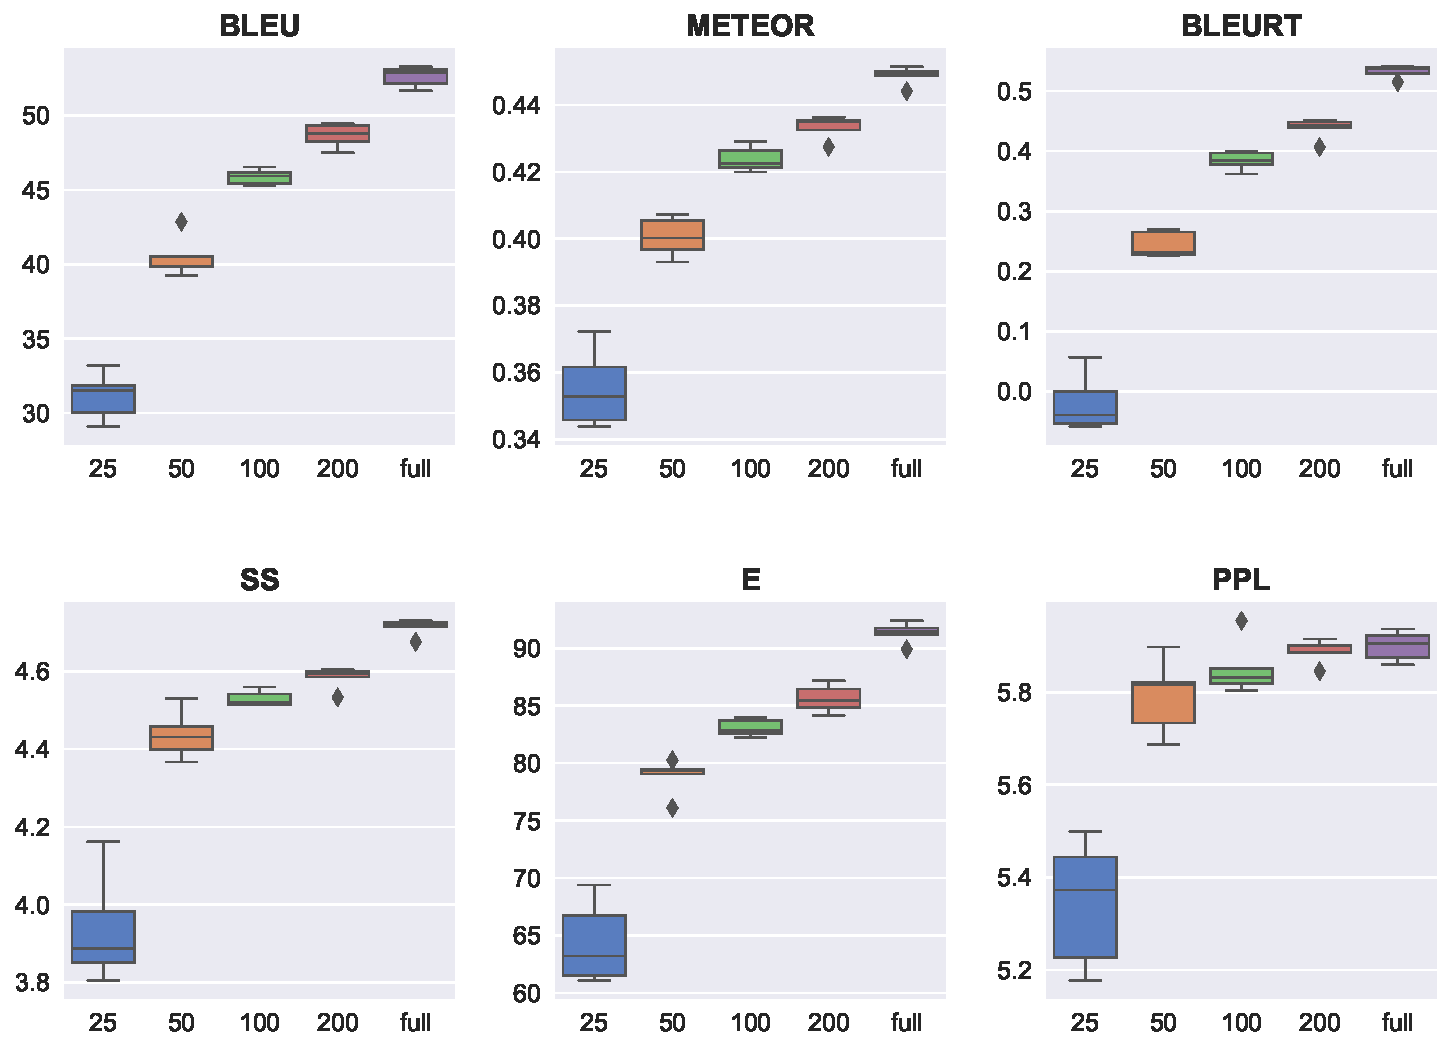
\includegraphics[width=0.7\textwidth]{img/rel2text-fewshot.pdf}
    \caption{Boxplots for selected metrics from Table \ref{tab:auto} w.r.t. the number of examples (displayed on the \textit{x}-axis, $\textit{full} = 1522$), taking into account variance from individual random seeds (cf.\ Table~\ref{tab:autostdev}).}\label{fig:fewshot}
\end{figure}


\begin{figure}[t]
    \centering
    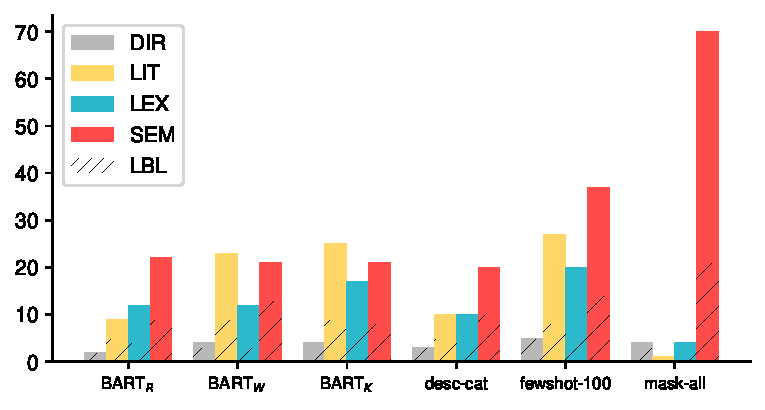
\includegraphics[width=0.7\textwidth]{img/rel2text-graph.pdf}
    \caption{Number of annotated errors per model (see §\ref{sec:manual} and Table~\ref{tab:cat} for the description of error categories and §\ref{sec:experiments} for the models). The striped part signifies that the label of the input was marked as unclear. See Appendix \ref{app:manual} for details.}\label{fig:manual}
\end{figure}




\section{Downstream Tasks}
\label{sec:downstream}
Given that the \BARTr{} model can describe relations from their labels with high accuracy, we investigate if we can use the model to replace manually created templates in downstream tasks. We select two qualitatively different tasks, both using the idea of transforming individual input triples to simple sentences as a preprocessing step: tabular reasoning (§\ref{sec:tab_res}) and zero-shot data-to-text generation (§\ref{sec:zeroshot}).

\subsection{Tabular Reasoning}
\label{sec:tab_res}

\citet{gupta2020infotabs} presented the \textsc{InfoTabS} dataset as an NLI benchmark on tabular data. Each example is a structured table with a set of premises, i.e.\ natural language claims about the table; the task is to determine whether each premise is entailed by the table, contradicted by it, or neither.

They represent the table as \textit{a paragraph} where each table cell is represented as a short sentence, mostly using a simple template \text{``The \textit{key} of \textit{title} are \textit{value}.''} \citet{neeraja2021incorporating} extend \citeauthor{gupta2020infotabs}'s approach, including a \textit{better paragraph representation} for which they prepare a fine-grained set of rules for individual entity categories. The rules\footnote{Formalized using more than 250 lines of Python code: \url{https://github.com/utahnlp/knowledge\_infotabs/blob/main/scripts/preprocess/bpr.py\#L120}} aim to minimize the number of ungrammatical sentences and improve the reasoning abilities of the NLI model.

We replicate the setup of \citet{neeraja2021incorporating} for the original (OPR) and better (BPR) paragraph representation using their public codebase. We then replace their templates with our \BARTr{} model, verbalizing the triple (\textit{title}, \textit{key}, \textit{value}). The results are summarized in Table \ref{tab:nli}.

\begin{table}[t]\centering
    \small
    \setlength{\tabcolsep}{4pt}
    \begin{tabular}{lcccc}\toprule
        premise repr.                       & dev   & $\alpha_1$ & $\alpha_2$ & $\alpha_3$ \\\midrule
        OPR \cite{gupta2020infotabs}        & 76.78 & 75.30      & 68.46      & 64.63      \\
        BPR \cite{neeraja2021incorporating} & 77.04 & 74.44      & 67.46      & 63.17      \\
        \BARTr{} (ours)                     & 74.44 & 74.31      & 64.59      & 63.46      \\
        \bottomrule
    \end{tabular}
    \caption{Accuracy for the dev set and test sets  $\alpha_{1,2,3}$ from the \textsc{InfoTabS} dataset. The results are averaged over 3 random seeds.}\label{tab:nli}
\end{table}

Our preliminary manual evaluation suggests that the sentences from our model are indeed more grammatical (even compared to BPR). However, we observe that the
performance is comparable across all three test sets. In line with \citet{mccoy2019right}, we conclude that for classification tasks such as NLI, the input content appears to be more important than the input form.

\subsection{Zero-shot Data-to-Text Generation}
\label{sec:zeroshot}

\citet{kasner2022neural} proposed a setup for zero-shot D2T generation in which pretrained models are used to gradually transform text into the final description. The first step of the pipeline requires transforming individual triples into text. We focus on the WebNLG dataset, for which the authors manually created 354 templates.\footnote{Available at \url{https://github.com/kasnerz/zeroshot-d2t-pipeline/blob/main/templates/templates-webnlg.json}} We replicate the authors' setup using their public code, applying \BARTr{} instead of the templates.
The results are summarized in Table \ref{tab:zeroshot}.

\begin{table}[t]\centering
    \small
    \setlength{\tabcolsep}{4pt}
    \begin{tabular}{clcccc}\toprule
        dataset                            & model    & BLEU  & METEOR & O     & H     \\\midrule
        \multirow{2}{*}{\textit{filtered}} & orig     & 43.19 & 39.13  & 0.152 & 0.073 \\
                                           & \BARTr{} & 45.39 & 38.97  & 0.056 & 0.161 \\\cdashlinelr{1-6}
        \multirow{2}{*}{\textit{full}}     & orig     & 42.92 & 39.07  & 0.051 & 0.148 \\
                                           & \BARTr{} & 44.63 & 38.93  & 0.058 & 0.166 \\
        \bottomrule
    \end{tabular}
    \caption{Lexical similarity metrics (BLEU, METEOR) and ommission (O) and hallucinaton (H) rate; following the setup in \citet{kasner2022neural}.}\label{tab:zeroshot}
\end{table}

We note that the pipeline using our model for preprocessing is able to achieve improvements of $\sim$2 BLEU points, at the cost of a slightly higher omission and hallucination rate, but crucially without needing the manual effort to create templates.
Cursory examination shows that sentences produced by our model are qualitatively similar to the manual templates, but more varied. Unlike the templates, our model may verbalize a relation differently depending on the context.
Overall, we argue that training a PLM on verbalizing individual relations can potentially replace the manual effort of creating simple templates, which will have a notable impact for scaling similar approaches to larger datasets.





\section{Describing Data in Common Formats}
\label{sec:quintd}